% !TeX program = lualatex
% !TeX encoding = utf8
% !TeX spellcheck = uk_UA
% !TeX root =../FTProblems.tex

%=========================================================
\Opensolutionfile{answer}[\currfilebase/\currfilebase-Answers]
\Writetofile{answer}{\protect\section*{\nameref*{\currfilebase}}}
\chapter{Квазістаціонарні поля і струми}\label{\currfilebase}
%=========================================================

\begin{Theory}
	Kвазістаціонарними називають поля, які виникають за умов, коли можна знехтувати струмами зміщення. Нижче квазістаціонарні поля буде розглянуто на прикладі розрахунків скін ефекту.

	Умови квазистаціонарності в провідниках виконуються, коли провідність  $\lambda \gg \omega$, де $\omega$~--- характерна частота змін поля. Зовні провідників умова  квазістаціонарності  виконується, коли просторовий масштаб системи, що розглядається, значно менший за характерну довжину хвилі випромінювання, пов'язаною з процесом.

	Скін-ефект --- явище проникнення електромагнітного поля в провідник на певну глибину, яка називається скін-шар. Скін-ефект призводить до протікання струму в провіднику в основному в області скін-шару, і, як наслідок, збільшення опору провідника. При скін-ефекті змінний струм високої частоти протікає переважно лише в поверхневому шарі.

	Усередині однорідного провідника з рівнянь Максвелла для квазістаціонарного поля випливають рівняння:
	\begin{equation}
		\begin{aligned}\label{eq:skin-effect}
			\Delta \Hfield & = \frac{4\pi\mu\lambda}{c^2}\frac{\partial\Hfield}{\partial t},  \\
			\Delta \Efield & = \frac{4\pi\mu\lambda}{c^2}\frac{\partial\Efield}{\partial t} ,
		\end{aligned}
	\end{equation}
	де $\lambda$~--- провідність,  $\mu$~---магнітна проникність.

	Глибина проникнення електричного поля у провідник (товщина скін-шару) визначається формулою:
	\begin{equation}\label{eq:skin-thickness}
		\delta = \frac{c}{\sqrt{2\pi\mu\lambda\omega}}.
	\end{equation}
    В задачах цього підрозділу вважати $\epsilon=\mu=1$.
\end{Theory}

\section{Розтікання зарядів в провідниках. Струми Фуко}

%=========================================================
%\begin{problem}
%Струми та заряди зосереджені між двома площинами $x = 0$  та $x = a$. Середнє значення за часом від густини заряду  $\left\langle \rho\right\rangle_t =0 $ у будь-якій точці. Густина струму є:
%\begin{align*}
%	\vect{j} & = j_0\vect{e}_x \left( 1-\frac{x}{a}\right) \frac{x}{a}\cos\omega t, \quad x \in \left[ 0, a\right] \\
%	\vect{j} & = 0, \quad x \notin \left[ 0, a\right],
%\end{align*}
%де $j_0=\const$, $\vect{e}_x$ --- одиничний вектор осі абсцис. Знайти густину заряду $\rho(x, y, z, t)$.
%\end{problem}

%=========================================================
\begin{problem}
Електричне поле $\Efield = f(x)\vect{e}_ze^{- i\omega t} $  паралельне площині $x = 0$, що розділяє метал та вакуум. Провідність металу $\lambda$ . На межі розділу  $f(0) = E_0$, усередині металу  $f(\infty) = 0$  Знайти розподіл густини струму.
\end{problem}

%=========================================================
\begin{problem}
У початковий момент електрони з концентрацією $n_0$   знаходяться в спокої і рівномірно розподілені усередині пласкої області товщиною $2a$. При $t>0$  вони починають рухатися під дією власного (усередненого) електричного поля. Знайти закон спадання густини заряду в центрі області~$\rho(0,t)$.
\begin{solution}
	Передусім відзначимо, що тут ми розглядаємо ідеальну картину з неперервним рівномірним розподілом густини заряду, як це зазвичай прийнято в макроскопічній електродинаміці. Виберемо систему декартових координат з абсцисою ортогонально до початкового шару.

	Нехай $X(x,t)$~--- траєкторія частинки, яка при $t = 0$   мала координату $x$ , тобто $X(0,t) = x$. Напруженість поля зростає монотонно по $x$, відповідно, швидкість і прискорення кожної частинки~--- також. Тому <<задні>> частинки не наздоганяють <<передні>>, тобто  $X(x_1,t) > X(x_2,t)$  при ${x_1} > {x_2}$.



		Оскільки поле плаского шару ~--- однорідне у просторі, це означає, що на кожну частинку весь час діє одне і теж саме електричне поле:
		\[
			\frac{{{\partial ^2}X(x,t)}}{{\partial {t^2}}} = \frac{e}{m_e}E(x) = \omega _p^2x,
		\]
		\[
			\omega _p^2 = \frac{{4\pi {e^2}{n_0}}}{m_e},
		\]
	$m_e$~--- маса електрона. Поле однорідного шару визначено за теоремою Гаусса.

		З рівнянь рівноприскореного руху:
		\[
			X(x,t) = x\left[ {1 + \omega _p^2\frac{{{t^2}}}{2}} \right]
		\]
		видно, що розподіл частинок весь час пропорційний початковому положенню.


		Положення крайніх частинок $X(a,t) = a\left[ {1 + \omega _p^2\frac{{{t^2}}}{2}} \right]$.

        \clearpage

	Густина у будь-якій точці шару, що розширюється, є
	\[
		\rho (x,t) = e{n_0}{\left[ {1 + \omega _p^2\frac{{{t^2}}}{2}} \right]^{ - 1}}\theta \left[ {X(a,t) - x} \right].
	\]
\end{solution}
\end{problem}


%=========================================================
\begin{problem}[Максвеллівська релаксація]\label{prb:MaxwellRelax}
Пласка нескінченна однорідна плита має діелектричну проникність $\epsilon_1$  і провідність $\lambda_1$ і розташована між площинами $x = 0$  і $x = a$ (декартові координати). Навколо плити ідеальний ізолятор. У початковий момент $t= 0$  вільний заряд з густиною $\rho_1$  рівномірно розподілений всередині плити, на поверхні та зовні плити вільних зарядів немає. При  $t > 0 $ починається квазистаціонарне перетікання зарядів, причому утворюється вільний поверхневий заряд густиною $\sigma(t)$  на границях плити. Виконується закон Ома  $\vect{j} = \lambda\Efield$. Знайти  $\sigma(t)$  а також розподіл густини струму $\vect{j}(x,t)$ всередині плити.
\begin{solution}
	Всередині плити відбувається розтікання заряду (максвелівська релаксація), яке має місце за умови виконання закону Ома. А саме, з рівняння неперервності, закону Ома та рівняння Максвелла $\vect{\nabla}\cdot\Efield = -4\pi\rho$   випливає:
	\[
		\rho (x,t) = \rho_1\exp \left(  - \frac{4\pi \lambda _1}{\epsilon _1}t \right).
	\]

	Для плаского розподілу заряду поле спрямовано по осі $x$. З рівняння Максвелла маємо:
	\[
		E_x(x,t) = 4\pi \left( {x - \frac{a}{2}} \right)\frac{{{\rho_1}}}{{{\epsilon _1}}}\exp \left( { - \frac{{4\pi {\lambda _1}}}{{{\epsilon_1}}}t} \right),
	\]
	звідки, за законом Ома:
	\[
		\vect{j}(x,t) = 4\pi \vect{e}_x\left( x - \frac{a}{2} \right)\frac{\lambda _1\rho _1}{\epsilon _1}\exp \left( - \frac{4\pi\lambda_1}{\epsilon_1}t \right).
	\]

	Заряд, що був всередині, з часом порівну розподіляється між двома поверхнями плити і на кожній з них

	\[
		\sigma (t) = \frac{a\rho_1}{2}\left[ {1 - \exp \left( { - \frac{{4\pi {\lambda _1}}}{{{\varepsilon _1}}}t} \right)} \right].
	\]
	%Звідси видно, що знак $\sigma(t)$  за малих $t$ визначається співвідношенням  $\lambda_1/\epsilon_1$ і  $\lambda_2/\epsilon_2$. Наприклад, якщо середовище зовні плити ізолятор $\lambda _2/\epsilon_2 \ll  \lambda_1/\epsilon_1$, спочатку майже весь заряд зосереджується на поверхні, а потім повільно спадає.
\end{solution}
\end{problem}

%=========================================================
\begin{problem}
Нескінченний однорідний циліндр радіуса $R$ має діелектричну проникність $\epsilon_1$  і провідність $\lambda_1$. Навколо~--- ідеальний ізолятор. У початковий момент $t = 0$ вільний заряд з густиною $\rho_1$ рівномірно розподілений всередині циліндра, на поверхні та зовні вільних зарядів немає. При $t > 0$  починається квазістаціонарне перетікання зарядів, причому утворюється вільний заряд з поверхневою густиною $\sigma(t)$  на поверхні циліндра. Виконується закон Ома   $\vect{j} = \lambda\Efield$. Знайти  $\sigma(t)$ та розподіл густини струму $\vect{j}(\vect{r},t)$  всередині циліндра.
\begin{solution}
	Задача аналогічна~\ref{prb:MaxwellRelax}. З урахуванням циліндричної симетрії задачі видно, що напруженість електричного поля має лише радіальну (перпендикулярну до осі циліндра) компоненту. З інтегральної форми рівнянь Максвелла в середовищі маємо:
	\[
		\Efield({\vect{r}},t) = 2\pi {\vect{r}}\frac{{{\rho _1}}}{{{\epsilon _1}}}\exp \left( { - \frac{{4\pi {\lambda _1}}}{{{\epsilon_1}}}t} \right),
	\]
	звідки
	\[
		\vect{j}(\vect{r},t) = 2\pi \vect{r}\frac{{{\lambda_1}{\rho_1}}}{{{\epsilon_1}}}\exp \left( { - \frac{{4\pi {\lambda _1}}}{{{\epsilon _1}}}t} \right).
	\]
	Для поверхневої густини заряду маємо:
	\[
		\sigma (t) = \frac{{R{\rho _1}}}{2}\left[ {1 - \exp \left( { - \frac{{4\pi {\lambda _1}}}{{{\varepsilon _1}}}t} \right)} \right].
	\]
\end{solution}
\end{problem}

%=========================================================
\begin{problem}
Однорідна куля радіуса $R$ має діелектричну проникність $\epsilon_1$  і провідність $\lambda_1$. Навколо~--- ідеальний ізолятор. У початковий момент $t = 0$ вільний заряд з густиною $\rho_1$ рівномірно розподілений всередині куля, на поверхні та зовні вільних зарядів немає. При $t > 0$  починається квазістаціонарне перетікання зарядів, причому утворюється вільний заряд з поверхневою густиною $\sigma(t)$  на поверхні кулі. Виконується закон Ома   $\vect{j} = \lambda\Efield$. Знайти  $\sigma(t)$ та розподіл густини струму $\vect{j}(\vect{r},t)$  всередині кулі.
\begin{solution}
	Всередині кулі маємо:
	\[
		\rho (t) = {\rho _1}\exp \left( { - \frac{{4\pi {\lambda_1}}}{{{\varepsilon _1}}}t} \right).
	\]
	Заряд зосереджується на поверхні кулі з густиною:
	\[
		\sigma (t) = \frac{{R{\rho _1}}}{3}\left[ {1 - \exp \left( { - \frac{{4\pi {\lambda _1}}}{{{\varepsilon _1}}}t} \right)} \right].
	\]
	З урахуванням сферичної симетрії задачі (напруженість електричного в окремій точці спрямована по радіусу) та з інтегральної форми рівнянь Максвелла в середовищі отримуємо напруженість поля. Густина струму:
	\[
		\vect{j}(\vect{r},t) = 4\pi \vect{r}\frac{{{\lambda_1}{\rho _1}}}{{3{\epsilon _1}}}\exp \left( { - \frac{{4\pi {\lambda_1}}}{{{\epsilon _1}}}t} \right).
	\]
\end{solution}
\end{problem}


%=========================================================
\begin{problem}
Метал знаходиться в області $x \in [-a, a]$ , його провідність  $\lambda$. Електричне поле має вид  $\Efield = f(x)\vect{e}_z\exp ( - i\omega t)$. На границях  $f( - a) = f(a) = E_0$ . Знайти розподіл густини струму.
\end{problem}

%=========================================================
\begin{problem}\label{prb:TrueSkin}
    Вздовж нескінченного циліндричного провідника радіуса $a$, матеріал якого має провідність $\lambda$ і магнітну проникність $\mu$,  тече змінний струм $I = I_0e^{-i\omega t}$. Зовні провідника~--- вакуум. Знайдіть розподіл густини струму та її асимптотику за високих частот.
\begin{solution}
    Використавши  рівняння для електричного поля~\label{eq:skin-effect} в циліндричних координатах та закон Ома отримаємо рівняння для густини струму:
\[
		\frac{1}{r}\frac{\partial }{{\partial r}}\left( {r\frac{{\partial {j_z}}}{{\partial r}}} \right) + {k^2}{j_z} = 0, \quad k^2 = \frac{4i\pi\lambda\mu\omega}{c^2} = \frac{2i}{\delta^2}.
\]

Розв'язком цього рівняння є функція вигляду $j_z = AJ_0(kr) + BN_0(kr)$. Оскільки $\lim\limits_{r\to0}N_0(kr) = -\infty$, то стала $B = 0$. Сталу $A$ можна знайти знаючи амплітуду струму
\[
   I_0 = \int\limits_0^a j_z(r)\ 2\pi rdr = 2\pi A \int\limits_0^a r J_0(kr) dr = 2\pi A \frac{a}{k} J_1(ka),
\]
отже, густина струму
\[
	j_z = \frac{k}{2\pi a} \frac{J_0(kr)}{J_1(ka)} I_0e^{-i\omega t}.
\]
За великих частот $ka \gg 1$ та в області біля краю провідника $ r \lessapprox a$ (див. формулу~\eqref{eq:Jxgg1}) маємо:
\[
    j_z = \frac{1-i}{2\pi\delta} I_0 \sqrt{\frac1{ar}} e^{\left( \frac{i - 1}{\delta} (a-r) - i\omega t\right) }.
\]

Дійсна амплітуда густини струму має вигляд:
\[
    j_0(r) = \frac{I_0\sqrt{2}}{2\pi\delta}  \sqrt{\frac1{ar}}e^{\frac{r-a}{\delta}},
\]
графічне зображення зображення цієї залежності подано на рисунку

\begin{center}
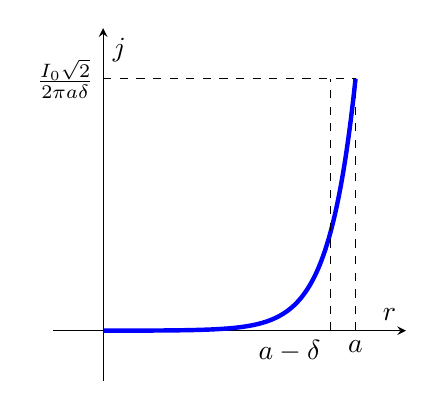
\begin{tikzpicture}
\begin{axis}%
[
            clip=false,
			axis lines = middle,
			axis line style={-stealth},
			% === Підпис координатних осей ===
            xtick = \empty,
            ytick = \empty,
			xlabel={$r$},
			ylabel={$j$},
		    % === Налаштування розміру графіка ===
   			width=0.5\linewidth,
   			height=0.5\linewidth,
   			% === Розширення границь осей ===
   			enlargelimits={abs=0.2},
]

\addplot[blue, domain=0:1, samples=500, ultra thick] {sqrt(1/x)*e^(-(1-x)/(1e-1))};
\draw[dashed] (axis cs:1,0) node[below] {$a$} -- (axis cs:1,1);
\draw[dashed] (axis cs:0.9,0) node[below left] {$a-\delta$} -- (axis cs:0.9,1);
\draw[dashed] (axis cs:0,1) node[left] {$\frac{I_0\sqrt{2}}{2\pi a\delta} $} -- (axis cs:1,1);
\end{axis}
\end{tikzpicture}
\end{center}
\end{solution}
\end{problem}

%=========================================================
\begin{problem}
    Обчисліть активний опір на одиницю довжини циліндричного провідника радіуса $a$ провідністю $\lambda$. Отримайте значення цієї величини за малих та за великих частот.
\begin{solution}
Густина струму в циліндричному провіднику (див. розв'язок до задачі~\ref{prb:TrueSkin})
\[
	j_z = \frac{k}{2\pi a} \frac{J_0(kr)}{J_1(ka)} I_0e^{-i\omega t}.
\]

Опір будемо шукати як $R = \frac{\left\langle Q \right\rangle }{\frac12I_0^2}$.


Із закону Джоуля-Ленца розрахуємо теплоту, яка виділяється в провіднику як%
%\footnote{Використано співвідношення \href{https://www.wolframalpha.com/input/?i=integrate+from+0+to+a+besselJ0\%28k*x\%29*besselJ0\%28Conjugate\%28k\%29*x\%29+x+dx}{$\int\limits_0^a  J_0(kr)J_0(k^*r) r dr = \frac{kJ_1(ka)J_0(k^*a) - k^*J_1(k^*a)J_0(ka)}{k^2-k^{*2}} $} (в додатках нема)}

\begin{multline*}
    \left\langle Q \right\rangle = \frac1{2\lambda}\int\limits_0^a \left| j_z^2\right| 2\pi r dr = \frac{2\pi}{2(2\pi a)^2} \frac{I_0^2}{\lambda} \frac{|k|^2}{J_1(ka)J_1(k^*a)}  \int\limits_0^a  J_0(kr)J_0(k^*r) r dr = \\
    = \frac{2\pi a}{2(2\pi a)^2} \frac{I_0^2}{\lambda} \frac{|k|^2}{J_1(ka)J_1(k^*a)} \frac{kJ_1(ka)J_0(k^*a) - k^*J_1(k^*a)J_0(ka)}{k^2-k^{*2}} =\\
    = \frac{2\pi a }{2(2\pi a)^2} \frac{I_0^2}{\lambda} \frac{|k|^2\delta^2}{4i}\left( \frac{kJ_0(k^*a)}{J_1(k^*a)} - \frac{k^*J_0(ka)}{J_1(ka)}\right) = \\ = \frac{2\pi a}{2(2\pi a)^2} \frac{I_0^2}{\lambda} \frac12  \left( \frac{k^*J_0(k^*a)}{J_1(k^*a)} + \frac{kJ_0(ka)}{J_1(ka)}\right) =  \frac{1}{4\pi a} \frac{I_0^2}{\lambda}  \mathrm{Re}\left(  \frac{kJ_0(ka)}{J_1(ka)} \right).
\end{multline*}

Отже
\[
    R = \frac{1}{2\pi a\lambda}  \mathrm{Re}\left[  \frac{kJ_0(ka)}{J_1(ka)} \right].
\]

Розглянемо випадок малих частот $|ka| \ll 1$:
\[
    R \approx \frac{1}{2\pi a\lambda}  \mathrm{Re} \left[k\left( 1 - \frac{k^2a^2}{4}\right)\frac{2}{ka}  \right] = \frac{1}{\pi a^2 \lambda}.
\]
Тобто, при малих частотах опір такий же, як і для для постійного струму.

Розглянемо випадок великих частот $|ka| \gg 1$:
\[
    R \approx \frac{1}{2\pi a\lambda} \mathrm{Re}\left[  ke^{k(r-a)} \right] \approx \frac{1}{2\pi a\lambda} \mathrm{Re}\left[  k(1-k(r-a)) \right] =  \frac{1}{2\pi a\delta\lambda}.
\]
З останньої формули випливає, що ефективна площа перерізу провідника в області великих частот дорівнює $2\pi a\delta$, тобто має дуже маленьку величину, зосереджену поблизу поверхні провідника.
\end{solution}
\end{problem}

%=========================================================
\begin{problem}\label{prb:BfieldTrueSkin}
    Для умов задачі~\ref{prb:TrueSkin} знайдіть розподіл магнітного поля всередині провідника.
\begin{solution}
    $B_{\phi_{\mathrm{in}}} = \frac{2}{cr} \int\limits_0^r j_z 2\pi r dt = \frac{2I}{ca} \frac{J_1(kr)}{J_1(ka)}$.
\end{solution}
\end{problem}


%=========================================================
\begin{problem}
        Обчисліть внутрішню індуктивність на одиницю довжини циліндричного провідника радіуса $a$ провідністю $\lambda$. Отримайте значення цієї величини за малих та за великих частот.
\begin{solution}
    Внутрішню індуктивність можна обчислити знаючи магнітне поле в середині провідника (див. відповідь до задачі~\ref{prb:BfieldTrueSkin})  виходячи з виразу $\frac{1}{4c^2}L_\mathrm{in}I^2 = \int\limits_0^a \frac{\left\langle  B_{\phi_{\mathrm{in}}}^2\right\rangle }{8\pi} 2\pi rdr$, маємо
    $L_\mathrm{in}  = -\frac{\delta^2}{2a}\left[ \frac{k^*J_0(ka)}{J_1(ka)} + \frac{kJ_0(k^*a)}{J_1(k^*a)}\right] $. За низьких частот $|ka| \ll 1$ внутрішня індуктивність  $L_\mathrm{in} = \frac12$, за великих частот $|ka| \gg 1$ --- $L_\mathrm{in} = \frac\delta a$.
\end{solution}
\end{problem}

%=========================================================
\begin{problem}
Всередині нескінченного циліндричного провідника радіуса $a$  діє електричне поле, паралельне осі $\Efield = \vect{e}_z f(r)e^{-i\omega t}$, невідома функція $f(r)$  залежить тільки від  відстані до осі циліндра $r$. Всередині провідника провідність $\lambda$, магнітна проникність $\mu = \const$. Знайдіть розподіл густини струму та її асимптотику за високих частот. Окремо оцініть відношення густини струму на осі провідника до значення при $r = a$, а також темп спадання біля краю.
%\begin{solution}
%Використаємо  рівняння для електричного поля~\label{eq:skin-effect}, яке в циліндричних координатах матиме вигляд:
%\[
%		\frac{1}{r}\frac{\partial }{{\partial r}}\left( {r\frac{{\partial {E_z}}}{{\partial r}}} \right) + {k^2}{j_z} = 0, \quad k^2 = \frac{4i\pi\lambda\mu\omega}{c^2} = \frac{2i}{\delta^2},
%\]
%що зводиться до рівняння для функції Бесселя $J_0$. Звідси, з урахуванням граничних умов для електричного поля при $r \ge  a$, а саме $\Efield = \Efield_0e^{-i\omega t}$, матимемо розв'язок
%\[
%    \Efield = \frac{J_0(kr)}{J_0(ka)}\Efield_0e^{-i\omega t},
%\]
%а для густини струму
%\[
%    \vect{j} = \frac{J_0(kr)}{J_0(ka)}\lambda\Efield_0e^{-i\omega t}.
%\]
%За високих частот $ka \gg 1$ матимемо
%\[
%    \vect{j} = \frac{}.
%\]
%\end{solution}
\end{problem}


%=========================================================
\begin{problem}\label{prb:Bat379}%Батыгин, 1970, №379
Нескінченний металевий циліндр, матеріал якого має провідність $\lambda$ і магнітну проникність $\mu$, розташований так, що його вісь збігається з віссю нескінченного соленоїда колового перерізу, по якому тече змінний струм $I = I_0e^{-i\omega t}$. Між циліндром і намоткою соленоїда, а також зовні соленоїда~--- вакуум. Знайдіть напруженість магнітного та індукційного електричного поля поля у всьому просторі, а також розподіл густини струму в циліндрі. Радіус циліндра дорівнює $a$, радіус соленоїда дорівнює $b$ ($a<b \ll c/\omega$), густина обмотки соленоїда $n$.
\begin{solution}
	Соленоїд створює однорідне магнітне поле, напрямлене по осі Z  всередині нього. Зовні соленоїда поле дорівнює нулю. За наявності циліндра в ньому виникають індукційні струми, що течуть по колам в площинах, ортогональних осі циліндра. Цю систему струмів можна розглядати як систему коаксіальних соленоїдів, поле яких не дає внесок зовні провідного  циліндра.

	Звідси магнітне поле $\Bfield = \Hfield = B_0\vect{e}_z$ при $r \in [a,b]$, де $B_0 = \frac{4\pi}{c}nI$, а зовні соленоїда (при $r > b$) $\Bfield = 0$.

	Усередині циліндра магнітне поле також напрямлене по осі $OZ$. Залежність усіх полів та струмів від часу така ж, як струм через обмотку.

	З рівнянь для квазістаціонарного поля (див. <<Теоретичні відомості, ф-ла ~\eqref{eq:skin-effect}>>) отримуємо
	\[
		\frac{1}{r}\frac{\partial }{{\partial r}}\left( {r\frac{{\partial {H_z}}}{{\partial r}}} \right) + {k^2}{H_z} = 0, \quad k^2 = \frac{4i\pi\lambda\mu\omega}{c^2} = \frac{2i}{\delta^2},
	\]
	що зводиться до рівняння для функції Бесселя $J_0$. Звідси, з урахуванням граничних умов для магнітного поля при $r = a$  та $r = b$, маємо
	\[H_z =
		\begin{cases}
			\frac{4\pi}{c}\frac{J_0(kr)}{J_0(ka)}nI_0e^{-i\omega t}, \quad r <a \\
			nI_0e^{-i\omega t}, \quad a \le r \le b                             \\
			0, r > b.
		\end{cases}
	\]

	Зауважимо, що $J_0(ka) \neq 0$, оскільки  $k$~--- комплексне, а нулі функції Бесселя лежать на дійсній осі.  З розкладу для  $J_0$  видно, що в формулу входить саме степені $k^2$, тому знак $k$ тут несуттєвий.

	При $r < a$, $\vect{j} = \frac{c}{4\pi}\rot\Hfield = \frac{c}{4\pi}\frac{d{H_z}}{dr}\left[ \vect{e}_r \times \vect{e}_z \right]$, звідки
	\[
		\vect{j} = knI_0\frac{J_1(kr)}{J_0(ka)}e^{-i\omega t}\vect{e}_{\phi},
	\]
	де використано що $J'_0(x) = -J_1(x)$. Використовуючи закон Ома $\Efield = \frac{\vect{j}}{\lambda}$, отримуємо електричне поле в середині провідника.
	Для областей $r >a$ та $r >b$ електричне поле можна знайти з рівняння Максвелла
	\[
		\frac{1}{r}\frac{\partial }{{\partial r}}\left( {r{E_\varphi }} \right) = \frac{{i\omega }}{c}{B_z} = \frac{{i\omega }}{c}{B_0}(t).
	\]

	Остаточно маємо
	\[
		E_{\phi} =
		\begin{cases}
			\frac{kcB_0}{4\pi\lambda}\frac{J_1(ka)}{J_0(ka)}e^{-i\omega t}, \quad r <a                                                                                        \\
			\frac{k}{\lambda}\frac{J_1(ka)}{J_0(ka)}\frac{a}{r}nI_0e^{-i\omega t} + \frac{4i\pi\omega }{2c^2r}\left( r^2 - a^2\right) nI_0e^{-i\omega t}, \quad a \le r \le b \\
			\frac{k}{\lambda}\frac{J_1(ka)}{J_0(ka)}\frac{a}{r}nI_0e^{-i\omega t} + \frac{4i\pi\omega }{2c^2r}\left( b^2 - a^2\right)nI_0e^{-i\omega t} , \quad r > b.
		\end{cases}
	\]
\end{solution}
\end{problem}


	%=========================================================
	\begin{problem}%Батыгин, 1970, №380
	Металевий циліндр радіусу $a$ внесли у зовнішнє однорідне магнітне поле  $\Bfield = \Bfield_0e^{-i\omega t}$, яке паралельне до його осі. Враховуючи результати задачі~\ref{prb:Bat379}, знайдіть густину струму всередині циліндру. Система знаходиться у вакуумі. Розгляньте окремо випадок великих та малих частот.
	\begin{solution}
		Розподіл полів і струму аналогічний задачі~\ref{prb:Bat379}, але тут немає соленоїду. Розв’язок шукаємо в циліндричних координатах у вигляді  $\Bfield(r) = f(r)\vect{e}_ze^{- i\omega t}$,  $\vect{e}_z$~--- одиничний вектор  осі $OZ$. Зовні циліндру є лише зовнішнє поле, тому  гранична умова для напруженості така $f(a) = B_0$ .

		Аналогічно до задачі~\ref{prb:Bat379} рівняння для магнітного поля за умови регулярності при $r = 0$ дає

		\[
			\Hfield(r) = \vect{e}_z{B_0}\frac{{{J_0}(kr)}}{{{J_0}(ka)}} e^{ - i\omega t},
		\]
		де $ k = \frac{1 + i}{\delta}$, $\delta = \frac{c}{\sqrt {2\pi \mu \lambda \omega}}$.

		Густину струму знайдемо з рівняння Максвела як
		\[
			\vect{j}=  - \frac{c}{4\pi}\frac{dH_z}{dr}\vect{e}_\phi = \vect{e}_\phi B_0\frac{kc}{4\pi }\frac{J_1(kr)}{J_0(ka)}e^{ - i\omega t}.
		\]

		Для малих частот $|ka| \ll 1$ (або $\delta \gg a$) маємо
		\[
			\vect{j} = \vect{e}_\phi\frac{\lambda \mu \omega ir}{{2c}}e^{ - i\omega t}.
		\]

		За високих частот $|ka| \gg 1$ (або $\delta \ll a$) в області $r \gg \delta$
		\[
			\vect{j}=  \vect{e}_\phi\frac{{c{B_0}(i - 1)}}{{4\pi \delta }}\sqrt {\frac{a}{r}} \exp \left[ { - \frac{{a - r}}{\delta }(1 - i) - i\omega t} \right].
		\]
		Тут використано асимптотичні формули для функцій Бесселя~\eqref{eq:Jxgg1}.
		%    З використанням закону Ома $\vect{j} = \lambda\Efield$ та закону Фарадея для області в середині провідника матимемо:
		%    \[
		%        2\pi r E_{\phi}(r) = - \frac1c \pi r^2 \dot{B}_z(t),
		%    \]
		%    звідки
		%    \[
		%        \vect{j}(r) = \frac{i\lambda\omega\mu H_0e^{-i\omega t} r}{2c}\vect{e}_{\phi}.
		%    \]
		%    Звідки, враховуючи результати задачі~\eqref{prb:Bat379}, маємо
		%
		%\[
		%    \vect{j}(r) = \frac{i\lambda\omega\mu H_0e^{-i\omega t} r}{2c}\vect{e}_{\phi}.
		%\]

		%    Для врахування явища самоіндукції (виникнення додаткового магнітного поля завдяки струмам Фуко) треба скористатись рівняннями~\eqref{eq:skin-effect}  в циліндричних координатах і використати граничні умови. В результаті будемо мати
		%   для а малих частот $|ka| \ll 1$ (або $\delta \gg a$):
		%	\[
		%		\vect{j}(r)  = \frac{i\lambda\omega B_0e^{-i\omega t}r}{2c}\vect{e}_{\phi},
		%	\]
		%	за великих частот $|ka| \gg 1$ (або $\delta \ll a$):
		%	\[
		%		\vect{j}(r) = (i - 1) \frac{cB_0e^{-i\omega t}}{2\pi\delta}\sqrt{\frac{a}{r}}e^{-(1+i)\frac{a-r}{\delta}}\vect{e}_{\phi}.
		%	\]
	\end{solution}
	\end{problem}

%=========================================================
\begin{problem}%Батыгин, 1970, №381
Яка кількість теплоти виділяється за період на одиницю довжини циліндра, розглянутого в задачі~\ref{prb:Bat379}. Дослідіть  випадок малих та високих частот.
\begin{solution}
	Використаємо формулу густини струму $j_{\phi} = knI_0\frac{J_1(kr)}{J_0(ka)}e^{-i\omega t}$, отриману в задачі~\ref{prb:Bat379}.

	Кількість теплоти, яка виділяється на одиницю довжини циліндра знайдемо як:
	\[
		Q = \frac{1}{2\lambda}\int\limits_0^a |j_{\phi}|^2 2\pi rdr.
	\]

	За малих частот $|ka| \ll 1$ (або $\delta \gg a$) маємо $j_{\phi} \approx nI_0\frac{k^2}{2}re^{-i\omega t} = inI_0\frac{r}{\delta^2}e^{-i\omega t}$ $\left( k^2 = \frac{2i}{\delta^2},\,  \delta = \frac{c}{\sqrt{2\pi\mu\lambda\omega}}\right) $, звідки
	\[
		Q = \frac{\pi n^2 I_0^2}{16\lambda}\left( \frac{a}{\delta}\right)^4.
	\]

	За високих частот $|ka| \gg 1$ (або $\delta \ll a$) основний внесок дає область поблизу поверхні циліндра, де можна застосувати асимптотичну формулу (див.~\eqref{eq:Jxgg1}) для густини струму
	\[
		j_{\phi} = nI_0\frac{i - 1}{\delta}\sqrt{\frac{a}{r}}e^{-(1-i)\frac{a-r}{\delta} - i\omega t},
	\]
	звідси
	\[
		Q = \frac{\pi n^2I_0^2}{\lambda}\left( \frac{a}{\delta}\right).
	\]
\end{solution}
\end{problem}


\section{Магнітні поля в надпровідниках}
\begin{Theory}
	Надпровідність~---явище протікання електричного струму у твердому тілі без втрат, тобто при строго нульовому електричному опорі тіла. Хоча надпровідність суттєво квантове явище, його феноменологічна теорія будується на основі класичних уявлень (теорія Лондонів).

	Згідно цієї теорії повні густини заряду та струму в надпровіднику складаються  з  нормальної та надпровідної частин:
	\[
		\rho = \rho_\text{над} + \rho_\text{норм}, \quad \vect{j} = \vect{j}_\text{над} + \vect{j}_\text{норм},
	\]
	де нормальна компонента густини струму $\vect{j}_\text{норм} = \sigma \Efield$ підпорядковується закону Ома.

	Електродинаміка надпровідників згідно теорії Лондонів описується матеріальними рівняннями вигляду:
	\begin{equation}\label{eq:London}
		c\rot{(\Lambda\vect{j}_\text{над})} + \Hfield =0, \quad
		\frac{\partial \vect{j}_\text{над}}{\partial t} - \frac{1}{\Lambda}\Efield = 0,
	\end{equation}
	де $\Lambda = \frac{m}{n_\text{над} e^2}$~--- параметр Лондонів, $n_\text{над}$~--- концентрація електронів, які забезпечують надпровідність.

	Надпровідність характеризується абсолютним діамагнетизмом. У магнітному полі в надпровідному матеріалі виникають такі струми, магнітне поле яких компенсує зовнішнє магнітне поле, тобто магнітне поле виштовхується із товщі надпровідника, воно проникає в провідник лише на невелику глибину, яка визначається за формулою:
	\begin{equation}\label{уйЖLondon_thickness}
		\delta = \sqrt{\frac{\Lambda c^2}{4\pi}}.
	\end{equation}
\end{Theory}

%=========================================================
\begin{problem}\label{prb:B341}%Батыгин, 1970, №341
Надпровідник заповнює півпростір $ x \ge 0$, при $x<0$~--- знаходиться вакуум. У вакуумі існує однорідне магнітне поле $\Hfield$ паралельне осі $OY$. Знайдіть розподіл магнітного поля і струмів на межі надпровідника в статичному випадку.
\begin{solution}
	$\Hfield = H_0e^{-\frac{x}{\delta}}\vect{e}_y$,
	$
		\vect{j} = -\frac{cH_0}{4\pi\delta}e^{-\frac{x}{\delta}}\vect{e}_z
	$.
\end{solution}
\end{problem}

%=========================================================
\begin{problem}
Надпровідна куля радіусу $R$ знаходиться в зовнішньому однорідному магнітному полі $H_0$. Знайдіть розподіл струмів і магнітне поле у всьому просторі.
%Розгляньте граничні випадки $R \gg \delta$ та $R \ll \delta$.
\begin{solution}
	Магнітне поле зовні кулі ($r > R$):
	\begin{align*}
		H_r = \left( H_0 + \frac{2m}{r^3}\right) \cos\theta, \\
		H_{\theta} = \left( - H_0 + \frac{m}{r^3}\right) \sin\theta,
	\end{align*}
	де
	\[
		m = -\frac{H_0R^3}{2}\left( 1 - 3\frac{\delta}{R}\cth\frac{R}{\delta} + 3\frac{\delta^2}{R^2}\right).
	\]

	Магнітне всередині кулі ($r < R$):
	\begin{align*}
		H_r = \frac{2\delta^2A}{r^3}\left[ \sh\frac{r}{\delta} - \frac{r}{\delta}\ch\frac{r}{\delta}\right]\cos\theta , \\
		H_{\theta} = \frac{\delta^2A}{r^3}\left[ \left( 1+ \frac{r^2}{\delta^2}\right) \sh\frac{r}{\delta} - \frac{r}{\delta}\ch\frac{r}{\delta}\right]\sin\theta,
	\end{align*}
	де
	\[
		A = - \frac32\frac{H_0R}{\sh\frac{R}{\delta} }.
	\]
\end{solution}
\end{problem}

%=========================================================
\begin{problem}%Батыгин, 1970, №344
Нескінченно довгий круглий циліндр радіуса $R$ з  надпровідника знаходиться в зовнішньому магнітному полі, яке напрямлене вздовж його осі симетрії. Знайдіть розподіл магнітного поля по об'єму циліндра та середній магнітний момент одиниці об'єму.
\begin{solution}
	$H_z = H_0\frac{I_0(r/\delta)}{I_0(R/\delta)}$,
	$\left\langle M_z\right\rangle  = -\frac{1}{4\pi}H_0\left( 1 - 2\frac{\delta}{R}\frac{I_1(r/\delta)}{I_0(R/\delta)}\right)$,
	де $I_0$ та $I_1$~--- модифіковані функції  Бесселя, $\delta$~--- глибина проникнення магнітного поля.
\end{solution}
\end{problem}

%=========================================================
\begin{problem}
В центр надпровідного кільця (без струму) індуктивністю $L$ і радіусом $R$ внесено магнітний диполь з
моментом $m$, який напрямлений вздовж осі кільця. Який струм установиться в кільці?
\begin{solution}
    Потік вектора магнітної індукції через довільну поверхню, що <<натягнута>> на кільце (тобто опирається на кільце), не залежить від вибору цієї поверхні. Далі обчислюємо потік через напівсферу радіуса R , що опирається на кільце.  Повний магнітний потік, що пронизує пронизує надпровідне кільце, зберігається $\Phi = \const$. Оскільки, в спочатку диполь не було внесено, $\Phi = 0$, і він залишатиметься таким же. Коли магнітний диполь опиниться в центрі кільця, повний магнітний потік, що пронизує кільце, є сумою потоку, створюваного струмом кільця, та потоку $\Phi_m$, створюваного диполем:
	\[
		\Phi = \frac1c LI + \Phi_m = 0,
	\]
	де $L$~-- індуктивність кільця, $I$~-- струм, що тече по кільцю.

Потік $\Phi_m$ через напівсферу легко обчислити, виходячи з формули для поля магнітного диполя, розташованого в центрі кільця:
\[
    \Bfield = \frac{3(\vect{m}\cdot\vect{r})\vect{r}- \vect{m}r^2}{r^5}.
\]

Обчислення потоку дає
\[
  \Phi_m = \frac{2\pi m}{R} .
\]
%
%
% $L_{21}$~-- коефіцієнт взаємоіндукції, $I_m$~-- умовний струм, що циркулює в диполі $p_m$ ($I_m = \frac{cp_m}{S}$, $S$~-- умовна площа витка диполя).
%
%	З закону збереження магнітного потоку випливає, що $I = - \frac{L_{12}}{L}\frac{cp_m}{S}$.
%	Для знаходження $L_{21}$, скористаємось теоремою взаємності, $L_{21} = L_{12} = \frac{2\pi S}{R}$.
	Звідси,
	\[
		I = - \frac{ 2\pi c m}{RL}.
	\]
	Знак мінус вказує на те, що індукційний що магнітний момент струму протилежний напрямку магнітного диполя.
\end{solution}
\end{problem}


%=========================================================
\begin{problem}
Провідне кільце з індуктивністю $L$ знаходиться в нормальному стані в зовнішньому магнітному полі (магнітний потік через контур кільця дорівнює $\Phi_0$). Потім температура знижується і кільце переходить в надпровідний стан. Який струм буде текти по кільцю, якщо вимкнути зовнішнє магнітне поле?
\begin{solution}
	$I = \frac{c\Phi_0}{L}$.
\end{solution}
\end{problem}

%=========================================================
\begin{problem}
У постійному однорідному магнітному полі з індукцією $B$ знаходиться кругле жорстке надпровідникове кільце радіусом $R$ малого перерізу. Коефіцієнт самоіндукцї кільця  $L$. У початковий момент площина кільця паралельна напрямку магнітного поля, а струм в кільці відсутній. Визначити силу струму в кільці відразу після того, як воно було повернуто так, що площина кільця стала перпендикулярна до ліній магнітного поля. Знайти витрачену роботу.
\begin{solution}
	$I = \frac{cB\pi R^2}{L}$, $A = \frac{\Phi^2}{2L} = \frac{B^2\pi^2 R^4}{2L}$.
\end{solution}
\end{problem}

%=========================================================
\begin{problem}
На якій висоті постійний магніт з магнітним моментом $p_m$ і масою $m$ буде левітувати положенні над плоскою горизонтальною поверхнею надпровідника? Магніт вважати точковим диполем. магнітний момент перпендикулярний площині.
\begin{solution}
	$h = \frac12 \sqrt[4]{\frac{3p_m^2}{mg}}$.
\end{solution}
\end{problem}

%=========================================================
%\begin{problem}
%Над плоскою поверхнею надпровідника I роду на ізолюючому шарі товщини $h = 5$~мм лежить тонке надпровідний кільце радіусом $R = 10$~см, по якому тече постійний струм. При якому струмі кільце почне левітувати над поверхнею надпровідника, якщо маса кільця $m = 1$~г?
%\begin{solution}
%	$I \ge c \sqrt{\frac{mgh}{2\pi R}} = 8.4\cdot 10^{10}$~Фр/с = $25$~А.
%\end{solution}
%\end{problem}

%=========================================================
\begin{problem}
Невелика надпровідна кулька радіусом $r$ знаходиться на осі на відстані $z$ від площини кільця радіусом $R$, по якому тече струм $I$; $\delta \ll r$. Знайдіть силу взаємодії між кулькою та кільцем.
\begin{solution}
    За умови $\delta \ll r$,   $F=\frac{6\pi^2 I^2 R^4 r^3 z}{(R^2+z^2)^4}$.
\end{solution}
\end{problem}


%=========================================================
%\begin{problem}
%Знайти розподіл магнітного тиску по поверхні надпровідної кулі радіусу $R$, що внесена в однорідне зовнішнє магнітне поле $\Bfield_0$.
%%\begin{solution}
%%	$ p = \frac{9}{32\pi} \Bfield_0\cdot\vect{r}$, де $\vect{r}$~--- радіус-вектор поверхні сфери.
%%\end{solution}
%\end{problem}


%=========================================================
\begin{problem}
Знайти силу, що діє на одиницю поверхні надпровідника, розглянутого в задачі~\ref{prb:B341}.
\begin{solution}
	$F_x = \frac{H_0^2}{8\pi}$.
\end{solution}
\end{problem}

\Closesolutionfile{answer}

